\graphicspath{{content/2_design/figures/}}
\section{Digital Motor Controller: Firmware}

\subsection{Flow Diagrams}

\begin{figure}[!htb]
    \centering
    \begin{minipage}{.45\textwidth}
        \centering
        \fbox{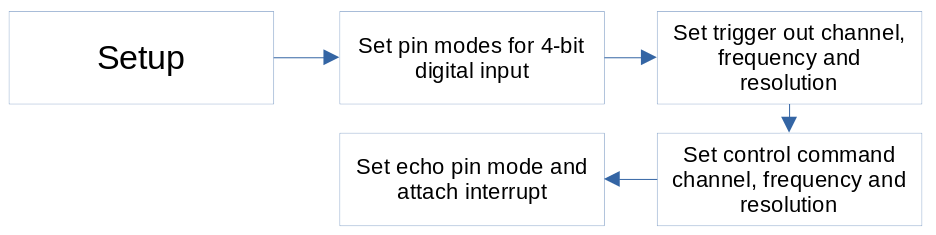
\includegraphics[width=0.9\linewidth]{digitalMotorController_flowChart_setup}}
        \captionof{figure}{Setup Diagram}
        \label{fig:digitalMotorController_flowChart_setup}
    \end{minipage}
    \begin{minipage}{.45\textwidth}
        \centering
        \fbox{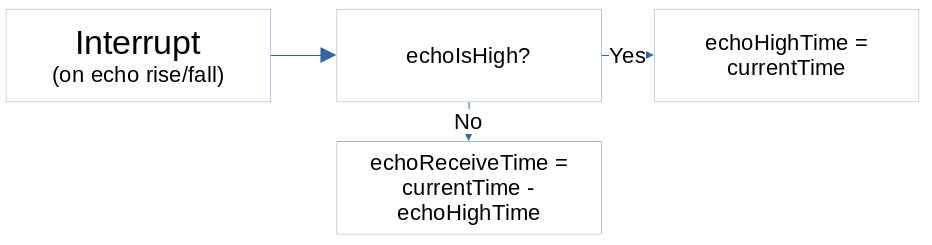
\includegraphics[width=0.9\linewidth]{digitalMotorController_flowChart_interrupt}}
        \captionof{figure}{Echo Interrupt Diagram}
        \label{fig:digitalMotorController_flowChart_interrupt}
    \end{minipage}
    \begin{minipage}{.45\textwidth}
        \centering
        \fbox{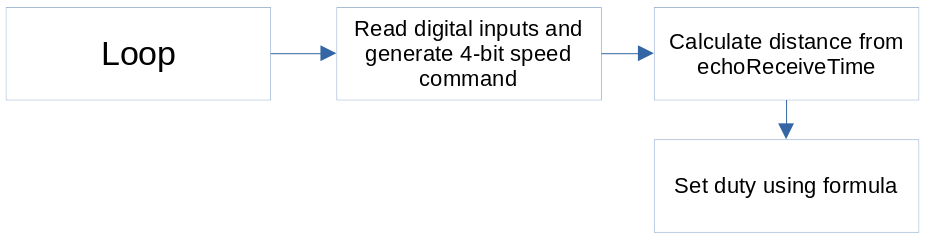
\includegraphics[width=0.9\linewidth]{digitalMotorController_flowChart_loop}}
        \captionof{figure}{Loop Diagram}
        \label{fig:digitalMotorController_flowChart_loop}
    \end{minipage}
\end{figure}

\subsection{Range Measurement}

As visible in the above flow diagram, range will be calculated by measuring the time that the echo pin is high. An interrupt will be used to detect when
the echo output changes from low to high, and vice versa. Then, this time will be divided by two and multiplied by the speed of sound to determine
the range of the object. Since the time distance will be in microseconds, the following formula may be used: $D = \frac{t_{us}}{2} \times \SI{343}{m \cdot s^{-1}} \times 10^{-6}$.

\subsection{PWM Control}

\subsubsection{Frequency}

If $f_{PWM}$ is too low, the motor switching will be noticeable. If it is too high, the MOSFET will not turn on fast enough.
The motor's resistance was measured as $R = \SI{5.3}{\ohm}$, and inductance was calculated as $L = \SI{1.6}{\milli\henry}$ using a frequency test.
The motor's cutoff frequency is therefore $f_c = \frac{R}{2 \pi L} = \frac{5.3}{2 \pi \times 1.6 \times 10^{-3}} \approx \SI{500}{Hz}$.
Since the FQD13N06L has a rise time of $t_{r(max)} = \SI{190}{ns}$, signals will only be affected at frequencies near $f_r = \frac{1}{\SI{190}{ns}} \approx \SI{5}{GHz}$.
$f_{PWM} = \SI{10}{kHz}$ could safely be chosen to ensure adequate filtering of wave harmonics, while not affecting switching times,
however $f_{PWM} = \SI{20}{kHz}$ is used to keep the switching frequency above human hearing.

\subsubsection{Formula}

The digital formula used should emulate the analog motor controller as closely as possible. The controller's range will therefore also be from 20 cm to 1 m
and will saturate at "digital rails". Given $S$, the 4-bit speed command, and $R$, the range, the following formulae may be used:
$C = \bar{R} - (1 - \bar{S})$ with $\bar{R} = \frac{R - R_{min}}{R_{max} - R_{min}}$ and $\bar{S} = \frac{S}{15}$.
Finally $duty = clamp(0, C, 1) \times controlResolution$. LEDC functions can then be used \cite{ledControl} to set this PWM appropriately.